\chapter{Preliminaries}\label{chapter:Preliminaries}

\section{Representation of Logic Circuits}
Independent of the underlying technology, digital circuits can be represented by logic functions. The Boolean Algebra, formed by mathematician George Boole in 1847, proposes these logic functions and provides a foundation to discuss about them.

\subsection{Boolean Functions}\label{subsec:boolfunc}
The definition as given here is based on an addition to Boolean calculus by Edward V. Huntington. CITE
The basis of a Boolean algebra is given as follows:

\begin{definition}[Basis for Boolean algebra]\label{Def:BasBool}
Given a finite set S, two binary functions · : S × S → S and + :
S × S → S, and one unary function ¬ : S → S, the tuple (S, ·,+,¬) is called a
Boolean algebra iff the following constraints hold for all a, b, c $\in$ S: \\

\centering
\begin{tabular}{l r l}

	     (1) & a · b = b · a & a + b = b + a \\

	     (2) &a · (b + c) = (a · b) + (a · c) & a + (b · c) = (a + b) · (a + c) \\
	     (3) & $\exists 1 \in S : a \cdot 1 = a$ &  $\exists 0 \in S : a + 0 = a$ \\
	     (4) &$\exists 0 \in S : a \cdot \neg a = 0$ & $\exists 1 \in S : a + \neg a = 1$. \\

\end{tabular}

\end{definition}

With the constraints describing (1) \textit{commutativity}, (2) \textit{distributivity}, (3) \textit{neutrality}, and (4)
\textit{complementarity}.\\

In the original definition a Boolean algebra is defined by the 6-tuple $(\mathbb{B}, \vee, \wedge, \neg, 0, 1)$, where $\vee$ and $\wedge$ are another denotations for the binary operands for disjunction $+$ and conjunction $\cdot$ in $\mathbb{B}$, the known unary negation function $\neg$, and two distinct elements 0 and 1. Negation $\neg a$ is also commonly notated as $\bar{a}$.\\

Since this definition is restricting the use of only the three Boolean functions $(\vee, \wedge, \neg)$, we want to extend by the following definition:

\begin{definition}
	A function $f : \mathbb{B}^n \to \mathbb{B}$, where $n \in N$, is called a Boolean function.
	Analogously, a
	function f : $\mathbb{B}^n \to \mathbb{B}^m$, where $n, m \in N$, is called multi-output Boolean function
	and can be interpreted as $f_v = (f_{v1}, . . . , f_{vm})$, where $f_{vi} : \mathbb{B}^n \to \mathbb{B}$, for all $1 \leq i \leq m$.
\end{definition}

A common notation for Boolean functions are the \textit{conjunctive normal form} (CNF) and \textit{disjunctive normal form} (DNF), using literals.

\begin{definition}
	A literal is an atom or the negation of an atom. In the former case the literal is positive, in the latter case it is negative.
\end{definition}

\begin{definition}
A formula F is in conjunctive normal form (CNF) if it is a
conjunction of disjunctions of literals:\\
\[\displaystyle\bigwedge_{i} \displaystyle\bigvee_{j} (\neg) v_{ij}, \]
where $v_{ij} \in \mathbb{B}$.\\
A formula F is in disjunctive normal form (DNF) if it is a
conjunction of disjunctions of literals:\\
\[ \displaystyle\bigvee_{i} \displaystyle\bigwedge_{j} (\neg) v_{ij}, \]
where $v_{ij} \in \mathbb{B}$.

\end{definition}

Using the CNF or rather the DNF and \textit{De Morgan's laws} following from the definitions in \ref{Def:BasBool}, it follows that any Boolean Algebra can be reduced to only two operands, e.g. conjunction ($\vee$) and negation ($\neg$). Any set of such two Boolean functions is called \textit{universal}.


\subsection{Logic Networks}

There are many ways of representing Boolean Functions. But most of them, including e.g. truth tables or reduced sum of products, suffer from drawbacks like exponential growth of size with the number of arguments and functions with exponential representations. The representation of combinational circuits as logic networks overcomes these restrictions and has proven to be very useful in the logic synthesis process. Following definition for directed acyclic graphs is shown in CITE:

\begin{definition}[Function graph]
	A function graph is a rooted, directed graph with vertex set $V$ containing two types of vertices. A \textit{nonterminal} vertex $v$ has as attributes an argument index $index(v) \in \{1, . . .,n\}$, and two children $low(v),high(v) \in V$. A \textit{terminal} vertex v has as attribute a value $value(v)\in\{0,1\}$.\\
	\\
	Furthermore, for any nonterminal vertex $v$, if $low(v)$ is also nonterminal, then we must have
	$index(v) < index(low(v))$. Similarly, if $high(v)$ is nonterminal, then we must have
	$index(v) < index(high(v))$.
\end{definition}

\begin{figure}
	\centering
	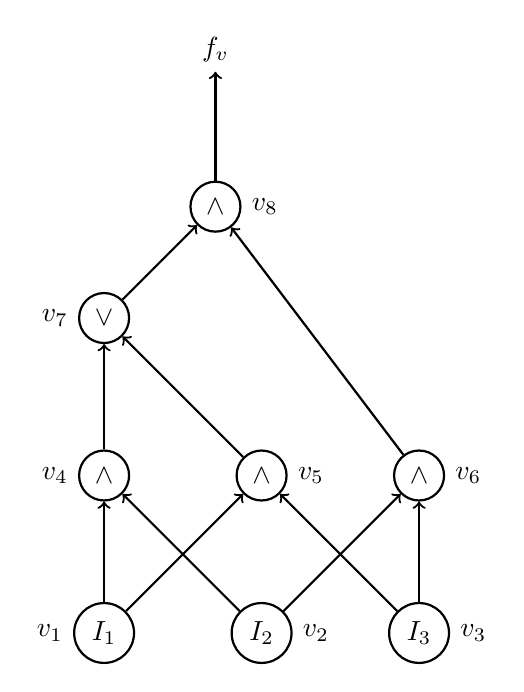
\begin{tikzpicture}[node distance={2cm and 2cm}, thick, main/.style = {draw, circle}] 
		\node[main] (1) [label=west:$v_1$]{$I_1$}; 
		\node[main] (2) [right of=1, label=east:$v_2$] {$I_2$};
		\node[main] (3) [right of=2, label=east:$v_3$] {$I_3$}; 
		
		\node[main] (4) [above of=1, label=west:$v_4$]{$\wedge$}; 
		\node[main] (5) [right of=4, label=east:$v_5$]{$\wedge$};
		\node[main] (6) [right of=5, label=east:$v_6$] {$\wedge$};
		
		\node[main] (7) [above of=4, label=west:$v_7$] {$\vee$};
		\node[main] (8) [above right of=7, label=east:$v_8$] {$\wedge$}; 
		\node [above of = 8] (f) {$f_v$};
		
		
		\draw[->] (1) -- (4);
		\draw[->] (1) -- (5);
		\draw[->] (2) -- (4);
		\draw[->] (2) -- (6);
		\draw[->] (3) -- (5);
		\draw[->] (3) -- (6);
		\draw[->] (4) -- (7);
		\draw[->] (5) -- (7);
		\draw[->] (7) -- (8);
		\draw[->] (6) -- (8);
		\draw[->] (8) -- (f);
		
	\end{tikzpicture} 
	\\
	\hfill \break
	The corresponding recursive Boolean functions read:\\
	\hfill \break
	\begin{tabular}{l l}
		
		$f_v = f_v(v_8)$ & $f_v(v_6) = f_v(v_2) \vee f_v(v_3)$ \\
		$f_v(v_8) = f_v(v_7) \wedge f_v(v_6)$ & $f_v(v_5) = f_v(v_3) \vee f_v(v_1)$ \\
		$f_v(v_7) = f_v(v_4) \wedge f_v(v_5)$ &  $f_v(v_4) = f_v(v_2) \vee f_v(v_1)$ \\
		&\\
		with primary inputs: & 	$f_v(v_1), f_v(v_2), f_v(v_3) \in \{0, 1\}$\\
		&\\
	\end{tabular}
	
	\caption{Binary Logic Network of Majority Function} \label{fig:LNMaj}
\end{figure}

Since the definition dosen't yet include Boolean Functions and reduces the number of children connected to a vertice to two, therefore only  allowing binary Boolean Functions, a custom definition is given:

\begin{definition}[Logic Network]
	A logic network is a rooted, directed graph with vertex set $V$ containing two types of vertices. A \textit{nonterminal} vertex $v$ has as attributes an argument index $index(v) \in \{1, . . .,n\}$, and $l$ children $child_1(v), ..., child_l(v) \in V$. A \textit{terminal} vertex v has as attribute a value $value(v)\in\{0,1\}$.\\
	\\
	Furthermore, for any nonterminal vertex $v$, if $child_i(v)$ with $ 1 \leq i \leq l$, then we must have
	$index(v) < index(child_i(v))$ respectively.
\end{definition}

\begin{definition}[Logic Network Boolean Functions]
	A set of nary Boolean Functions $\mathbb{B}$ is accessed via the argument index, assigning a Boolean Function $f_v$ to every vertex:
	\begin{enumerate}
		\item If v is a terminal vertex:
		\begin{enumerate}
			\item If $value(v)=1$, then $f_v=1$
			\item If $value(v)=0$, then $f_v=0$
		\end{enumerate}
		\item If $v$ is a nonterminal vertex with $index(v)=i$, then $f_v$ is the function \\ 
		$f_v(x_1, ..., x_n) = f_v(f_v(child_1(v)), ..., f_v(child_l(v)))$.
	\end{enumerate}
\end{definition}

The binary Logic Network of the ternary majority function is depicted figure \ref*{fig:LNMaj}:

\begin{definition}[Majority Function]
	The ternary Boolean majority function is defined as: $<a, b, c> = ab + ac + bc$, so that the function value equals the majority of it's incoming values.\\
	It follows: $<a, b, 0> = ab$ and $<a, b, 0> = a + b$.
\end{definition}

Because of the names used in the underlying libraries used to program the algorithms proposed in chapter... the vertices are referred to as nodes, while edges connecting a vertex with one of its children is called a signal. Terminal vertices, found at the beginning of the graph and therefore possessing the lowest indices, are called primary inputs. The enumerated vertices $f_{vi}$, representing the boolean functions are called primary outputs.\\
!!ADD a Denotation\\
As already mentioned in subsection \ref{subsec:boolfunc}, a set of two certain Boolean functions can form any Boolean algebra.
As long as this universality is contained the set of node functions can be extended. Using conjunction and negation as the only node functions of a logic network, we get the so called \textit{AND-Inverter Graphs} (AIGs). Another widely used binary logic network is the \textit{Majority-Inverter Graphs} (MIGs) utilizing the ternary majority function and negation. But there also exists a wide range of logic networks permitting more than just two node functions, like \textit{XOR-AND-Inverter Graphs} (XAGs).\\

Since the logic network represents the combinational circuit in the given technology, a suitable logic network representation has to be determined. Because, even though these logic networks can implement any Boolean function given in a specification, not every logic network can be synthesized into any given technology.
Looking at the current standard technology \textit{complementary metal-oxidesemiconductor} (CMOS), the logic network is then synthesized by using building blocks consisting of \textit{metal-oxide-semiconductor field-effect transistors} (MOSFETs), the elemental unit in this technology. The process of turning a circuit specification into a logic gate representation is called \textit{logic synthesis}.\\

Given these logic network characteristics, none of the representations are \textit{canonical}, which means that a given function can be represented by different logic networks. This property can be explained by the fact that nodes with the identity function are allowed. Even the exclusion of such identity nodes has no impact, since simple node combinations, like two negotiation nodes, collapse to the identity function. Following this argumentation, there exists an infinite number of logic networks representing one Boolean Function, resulting in he widely accepted assumption, that the determination of an optimal logic network is a $\mathcal{NP}$-complete problem. Attempts to create canonical logic networks, seem to evade this problem, but include co$\mathcal{NP}$-complete problems in itself. Algorithms used for logic synthesis are therefore based on approximate solutions.


\section{QCA Technology}

Following the well known Moores law CMOS technology is facing a multitude of challenges, e.g. short channel effect, impurity variations, and most importantly the heat, resulting from static and dynamic power losses. To tackle these challenges the International Roadmap for Devices and Systems (IDRS), former ITRS, proposes solutions within the semiconductor domain, e.g. new materials and multi-core architectures. But also new technologies are researched including Quantum computing and the domain of \textit{Field-Coupled Nanocomputing} (FCN). This work focuses on one of the most promising FCN technologies, namely \textit{Quantum dot cellular automata} (QCA). The main difference of this technology compared to CMOS is the representation of logical modes, using the location of electron pairs in QCA-cells, instead of voltage levels. Data between cells is transferred based on Coulomb repulsion, utilizing electromagnetic fields. This enables the technology to achieve high performance in terms of device density, clock frequency and power consumption.

Point out why majority gates are a big part of this technology. \\
Point out why wires and especially wire crossings are so expensive to produce. \\

\subsection{Cells}
As already mentioned, the elemental unit of this technology is a QCA-cell. Since there in no uniform way of build the quantum dots and connecting them to cells, we look at a rather lower-level abstraction depicted in figure \ref{fig:QCAStates}. The four circles in the corners of the QCA-cells show quantum-dots, that can be implemented by any charge container with discrete electrical energy states. Further a cell contains two excess electrons, which can be localized by the quantum dots. The energy barriers or the quantum dots are able to trap the charge of the electron. If an electron is trapped inside a quantum-dot it is filled black. Due to the Coulomb repulsion the electrons occupy diagonally opposed quantum dots,
resulting in two possible stable cell configurations and one unstable cell configuration.\\
A stable states indicates, that it is well distinguishable of the usual energy band and therefore has a energy difference to another stable state of minimum the thermal noise energy ($k_BT$). Only such states are suited for information transfer. The stable states can be derived from the cell Polarization, which can be $+1$ and $-1$ or $null$ in the unexcited state. The two stable states contain the same electrostatic energy and are used to encode the binary values $0$ and $1$.\\
In order to transfer information, cells are placed side by side, whereby the polarization of the driver cell, which is the left most cell inputting the information, changes the polarization of the adjacent cell. When the adjacent cell is polarized it can give its state to the next cell and so on. This simple structure is representing a wire in QCA-technology and its function is depicted in Figure \ref{fig:QCAWire}.

\begin{figure}
	\centering
	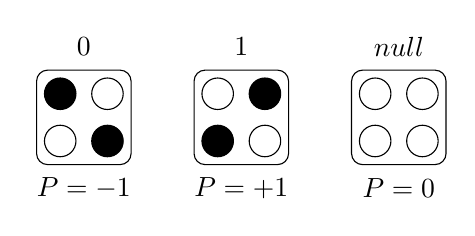
\begin{tikzpicture}
		%One QCA-Cell
		\node (A1) at (0.6,1.5) {$0$};
		\draw[rounded corners] (0, 0) rectangle (1.2, 1.2) [label=north:$v_7$]{};
		\node (A2) at (0.6,-0.3) {$P = -1$};
		
		\draw (0.3,0.3) circle (2mm);
		\draw [fill = black] (0.9,0.3) circle (2mm);
		\draw [fill = black](0.3,0.9) circle (2mm);
		\draw (0.9,0.9) circle (2mm);
		
		
		%One QCA-Cell
		\def\x{2}
		\node (B1) at (0.6+\x,1.5) {$1$};
		\draw[rounded corners] (\x, 0) rectangle (1.2 + \x, 1.2) {};
		\node (B2) at (0.6+\x,-0.3) {$P = +1$};
	
		\draw [fill = black] (0.3+\x,0.3) circle (2mm);
		\draw (0.9+\x,0.3) circle (2mm);
		\draw (0.3+\x,0.9) circle (2mm);
		\draw [fill = black] (0.9+\x,0.9) circle (2mm);
		
		
		%One QCA-Cell
		\def\x{4}
		\node (C1) at (0.6+\x,1.5) {$null$};
		\draw[rounded corners] (\x, 0) rectangle (1.2 + \x, 1.2) {};
		\node (C2) at (0.6+\x,-0.3) {$P = 0$};
		
		\draw (0.3+\x,0.3) circle (2mm);
		\draw (0.9+\x,0.3) circle (2mm);
		\draw (0.3+\x,0.9) circle (2mm);
		\draw (0.9+\x,0.9) circle (2mm);
		
		
	\end{tikzpicture} 

	\caption{QCA-Cell sates} \label{fig:QCAStates}
\end{figure}

\begin{figure}
	\centering
	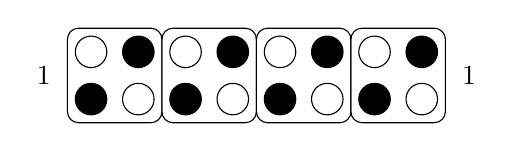
\begin{tikzpicture}
		%One QCA-Cell
		\node (A1) at (-0.3,0.6) {$1$};
		\draw[rounded corners] (0, 0) rectangle (1.2, 1.2) [label=north:$v_7$]{};
		
		\draw [fill = black](0.3,0.3) circle (2mm);
		\draw (0.9,0.3) circle (2mm);
		\draw (0.3,0.9) circle (2mm);
		\draw [fill = black](0.9,0.9) circle (2mm);
		
		
		%One QCA-Cell
		\def\x{1.2}
		\draw[rounded corners] (\x, 0) rectangle (1.2 + \x, 1.2) {};
		
		\draw [fill = black] (0.3+\x,0.3) circle (2mm);
		\draw (0.9+\x,0.3) circle (2mm);
		\draw (0.3+\x,0.9) circle (2mm);
		\draw [fill = black] (0.9+\x,0.9) circle (2mm);
		
		
		%One QCA-Cell
		\def\x{2.4}
		\draw[rounded corners] (\x, 0) rectangle (1.2 + \x, 1.2) {};
		\draw [fill = black](0.3+\x,0.3) circle (2mm);
		\draw (0.9+\x,0.3) circle (2mm);
		\draw (0.3+\x,0.9) circle (2mm);
		\draw [fill = black](0.9+\x,0.9) circle (2mm);
		
		%One QCA-Cell
		\def\x{3.6}
		\draw[rounded corners] (\x, 0) rectangle (1.2 + \x, 1.2) {};
		\draw [fill = black](0.3+\x,0.3) circle (2mm);
		\draw (0.9+\x,0.3) circle (2mm);
		\draw (0.3+\x,0.9) circle (2mm);
		\draw [fill = black](0.9+\x,0.9) circle (2mm);
		\node (C1) at (1.5+\x,0.6) {$1$};
		
		
	\end{tikzpicture} 
	
	\caption{Adjacent QCA-cells forming a wire} \label{fig:QCAWire}
\end{figure}

\subsection{Clocking}



\begin{figure}
	\centering
	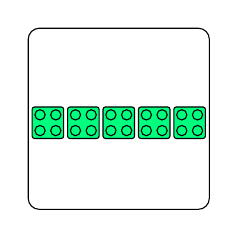
\begin{tikzpicture}
		\draw[rounded corners] (-0.05, -0.05 - 0.85) rectangle (2.3-0.05, 2.3-0.05 - 0.85){};
		\foreach \x/\xx in {0/0 ,0.4/0.05, 0.8/0.1, 1.2/0.15, 1.6/0.2}
		{
				
			\draw[rounded corners = 0.3mm, fill=SpringGreen] (\x + \xx, 0) rectangle (\xx + 1.2/3 + \x, 1.2/3){};
			\draw (0.3/3+ \x + \xx,0.3/3) circle (0.65mm);
			\draw (0.9/3+ \x + \xx,0.3/3) circle (0.65mm);
			\draw (0.3/3+ \x + \xx,0.9/3) circle (0.65mm);
			\draw (0.9/3+ \x + \xx,0.9/3) circle (0.65mm);
		}
	\end{tikzpicture}%
	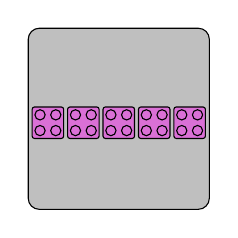
\begin{tikzpicture}
		\draw[rounded corners, fill=lightgray] (-0.05, -0.05 - 0.85) rectangle (2.3-0.05, 2.3-0.05 - 0.85){};
		\foreach \x/\xx in {0/0 ,0.4/0.05, 0.8/0.1, 1.2/0.15, 1.6/0.2}
		{
			
			\draw[rounded corners = 0.3mm, fill=Orchid] (\x + \xx, 0) rectangle (\xx + 1.2/3 + \x, 1.2/3){};
			\draw (0.3/3+ \x + \xx,0.3/3) circle (0.65mm);
			\draw (0.9/3+ \x + \xx,0.3/3) circle (0.65mm);
			\draw (0.3/3+ \x + \xx,0.9/3) circle (0.65mm);
			\draw (0.9/3+ \x + \xx,0.9/3) circle (0.65mm);
		}
	\end{tikzpicture}%
	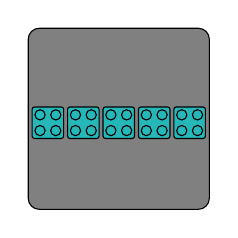
\begin{tikzpicture}
		\draw[rounded corners, fill=gray] (-0.05, -0.05 - 0.85) rectangle (2.3-0.05, 2.3-0.05 - 0.85){};
		\foreach \x/\xx in {0/0 ,0.4/0.05, 0.8/0.1, 1.2/0.15, 1.6/0.2}
		{
			
			\draw[rounded corners = 0.3mm, fill=BlueGreen] (\x + \xx, 0) rectangle (\xx + 1.2/3 + \x, 1.2/3){};
			\draw (0.3/3+ \x + \xx,0.3/3) circle (0.65mm);
			\draw (0.9/3+ \x + \xx,0.3/3) circle (0.65mm);
			\draw (0.3/3+ \x + \xx,0.9/3) circle (0.65mm);
			\draw (0.9/3+ \x + \xx,0.9/3) circle (0.65mm);
		}
	\end{tikzpicture}%
	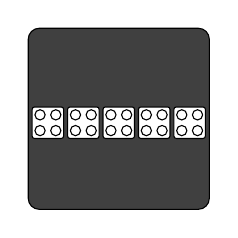
\begin{tikzpicture}
		\draw[rounded corners, fill=darkgray] (-0.05, -0.05 - 0.85) rectangle (2.3-0.05, 2.3-0.05 - 0.85){};
		\foreach \x/\xx in {0/0 ,0.4/0.05, 0.8/0.1, 1.2/0.15, 1.6/0.2}
		{
			
			\draw[rounded corners = 0.3mm, , fill=white] (\x + \xx, 0) rectangle (\xx + 1.2/3 + \x, 1.2/3){};
			\draw (0.3/3+ \x + \xx,0.3/3) circle (0.65mm);
			\draw (0.9/3+ \x + \xx,0.3/3) circle (0.65mm);
			\draw (0.3/3+ \x + \xx,0.9/3) circle (0.65mm);
			\draw (0.9/3+ \x + \xx,0.9/3) circle (0.65mm);
		}
	\end{tikzpicture}%
	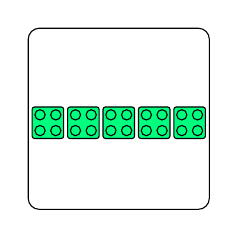
\begin{tikzpicture}
		\draw[rounded corners] (-0.05, -0.05 - 0.85) rectangle (2.3-0.05, 2.3-0.05 - 0.85){};
		\foreach \x/\xx in {0/0 ,0.4/0.05, 0.8/0.1, 1.2/0.15, 1.6/0.2}
		{
			
			\draw[rounded corners = 0.3mm, fill=SpringGreen] (\x + \xx, 0) rectangle (\xx + 1.2/3 + \x, 1.2/3){};
			\draw (0.3/3+ \x + \xx,0.3/3) circle (0.65mm);
			\draw (0.9/3+ \x + \xx,0.3/3) circle (0.65mm);
			\draw (0.3/3+ \x + \xx,0.9/3) circle (0.65mm);
			\draw (0.9/3+ \x + \xx,0.9/3) circle (0.65mm);
		}
	\end{tikzpicture}%
	
	\caption{QCA-Cell wire with corresponding clock zones} \label{fig:QCAClock}
\end{figure}

Explain the clocking of cells. \\
Show different clocking schemes and the ideas behind them. \\
Point out that one clocking zone is represented by exactly one cell and not multiple cells. \\
Point out the local and global clocking constraints

\subsection{Gates}
Talk about QCA Standard Cell Library

\subsubsection{Latches and Registers}



\section{P\&R problem}

Describe the challenges of P\&R in QCA, further details are in the next chapter